% --------------------------------------------------------------
% This is all preamble stuff that you don't have to worry about.
% Head down to where it says "Start here"
% --------------------------------------------------------------
 
\documentclass[10pt]{article}
 
\usepackage[margin=.3in, voffset=.3in, ]{geometry} 
\usepackage{amsmath,amsthm,amssymb, mathtools}
\usepackage{multicol}
\usepackage[subnum]{cases}
\usepackage{relsize}
\usepackage[makeroom]{cancel}
\usepackage[english]{babel}
\usepackage{graphicx}
\usepackage{calligra}
\usepackage[normalem]{ulem}
\usepackage{caption}
\usepackage{subcaption}
\usepackage{fancyhdr}
\usepackage{mathrsfs}
\usepackage{bbold}
\usepackage{physics}
\usepackage{tikz}
\usepackage{vwcol}

\DeclareMathAlphabet{\mathcalligra}{T1}{calligra}{m}{n} 
\DeclareFontShape{T1}{calligra}{m}{n}{<->s*[2.2]callig15}{}


% Makes '\sr' make a script r
\newcommand{\sr}{\ensuremath{\mathcalligra{r}}}
 
\newcommand{\N}{\mathbb{N}}
\newcommand{\Z}{\mathbb{Z}}
\newcommand{\ihat}{\boldsymbol{\hat{\textbf{\i}}}}
\newcommand{\jhat}{\boldsymbol{\hat{\textbf{\j}}}}
\newcommand{\khat}{\boldsymbol{\hat{\textbf{k}}}}
\newcommand{\rhat}{\boldsymbol{\hat{\textbf{r}}}}
\newcommand{\srhat}{\boldsymbol{\hat{\textbf{\sr}}}}
\newcommand{\xhat}{\boldsymbol{\hat{\textbf{x}}}}
\newcommand{\yhat}{\boldsymbol{\hat{\textbf{y}}}}
\newcommand{\zhat}{\boldsymbol{\hat{\textbf{z}}}}
\newcommand{\nhat}{\boldsymbol{\hat{\textbf{n}}}}
\newcommand{\phihat}{\boldsymbol{\hat{\textbf{$\phi$}}}}
\newcommand{\thetahat}{\boldsymbol{\hat{\textbf{$\theta$}}}}
\newcommand{\rhohat}{\boldsymbol{\hat{\textbf{$\rho$}}}}

\newcommand{\ve}[1]{\boldsymbol{\mathbf{#1}}}
\newcommand{\vect}[1]{\boldsymbol{\mathbf{#1}}}
\newcommand{\vc}[1]{\mathbf{#1}}
\newcommand{\fracl}[2]{\mathlarger{\frac{#1}{#2}}}
%\newcommand{\dd}{\, \mathrm{d}}
\newcommand{\eo}{\epsilon_0}
\newcommand{\mo}{\mu_\circ}
\newcommand{\tder}[2]{\frac{\dd #1}{\dd #2}}
\newcommand{\pder}[2]{\frac{\partial #1}{\partial #2}}
\newcommand{\dtder}[2]{\frac{\dd^2 #1}{\dd #2^2}}
\newcommand{\ttder}[2]{\frac{\dd^3 #1}{\dd #2^3}}
\newcommand{\dpder}[2]{\frac{\partial^2 #1}{\partial #2^2}}
\newcommand{\tpder}[2]{\frac{\partial^3 #1}{\partial #2^3}}
\newcommand{\intas}{ \int_{-\infty}^\infty}
\newcommand{\wt}[1]{\widetilde{#1}}
%\newcommand{\ev}[1]{\left\langle #1 \right\rangle}
%\newcommand{\ket}[1]{\left| #1 \right\rangle}
%\newcommand{\bra}[1]{\left\langle #1 \right|}
%\newcommand{\braket}[2]{\left\langle #1 \right| \left. \! #2 \right\rangle}
\newcommand{\ce}{\wt{\vect{E}}}
\newcommand{\cb}{\wt{\vect{B}}}
\newcommand{\K}{\frac{1}{4 \pi \eo}}
\newcommand{\lrp}[1]{\left( #1 \right)}
\newcommand{\lrb}[1]{\left[ #1 \right]}
\newcommand{\lrc}[1]{\left\{ #1 \right\}}
\newcommand{\evalb}[1]{\left. #1 \right|}
\newcommand{\herm}[1]{#1^\dagger}
 
\newenvironment{theorem}[2][Theorem]{\begin{trivlist}
\item[\hskip \labelsep {\bfseries #1}\hskip \labelsep {\bfseries #2.}]}{\end{trivlist}}
\newenvironment{lemma}[2][Lemma]{\begin{trivlist}
\item[\hskip \labelsep {\bfseries #1}\hskip \labelsep {\bfseries #2.}]}{\end{trivlist}}
\newenvironment{exercise}[2][Exercise]{\begin{trivlist}
\item[\hskip \labelsep {\bfseries #1}\hskip \labelsep {\bfseries #2.}]}{\end{trivlist}}
\newenvironment{problem}[2][Problem]{\begin{trivlist}
\item[\hskip \labelsep {\bfseries #1}\hskip \labelsep {\bfseries #2.}]}{\end{trivlist}}
\newenvironment{question}[2][Question]{\begin{trivlist}
\item[\hskip \labelsep {\bfseries #1}\hskip \labelsep {\bfseries #2.}]}{\end{trivlist}}
\newenvironment{corollary}[2][Corollary]{\begin{trivlist}
\item[\hskip \labelsep {\bfseries #1}\hskip \labelsep {\bfseries #2.}]}{\end{trivlist}}


\newenvironment{Figure}
  {\par\medskip\noindent\minipage{\linewidth}}
  {\endminipage\par\medskip}

\pagenumbering{gobble}

\ifx\du\undefined
	\newlength{\du}
\fi
\setlength{\du}{15\unitlength}

\pagestyle{fancy}
\lhead{Thermodynamics Equations}
\chead{MSU Comprehensive Exam 2016}
\rhead{Roy Smart}


 
\begin{document}

\begin{multicols}{2}
	\tiny
	\setlength{\abovedisplayskip}{-25pt}
	\setlength{\belowdisplayskip}{-25pt}
	\setlength{\abovedisplayshortskip}{0pt}
	\setlength{\belowdisplayshortskip}{0pt}
	\begin{align*}
	& \small \hspace{-10pt} \textbf{Equilibrium and State Quantities} \small \\
		& p V = NkT		\tag*{Ideal gas law (GNS. 1.2)} \\
		& p V = m N \frac{1}{3} \expval{\ve{v}^2} = \frac{2}{3} N \expval{\epsilon_{\text{kin}}}	\tag*{Kinetic theory of ideal gas (GNS. 1.10)} \\
		& \delta W = - p \: dV	\tag*{Infinitesimal work done by a change in volume (GNS. 1.20)} \\
		& \delta W = \mu \: dN	\tag*{Infinitesimal work done by adding a particle against potential $\mu$ (GNS. 1.24)} \\
		& \delta Q = C \: dT	\tag*{Infinitesimal heat added against heat capacity $C$ (GNS. 1.25)} \\
		& \lrb{p + \lrp{\frac{N}{V}}^2a}(V - Nb) = NkT	\tag*{Van de Waals' equation (GNS. 1.33)} \\
	& \small \hspace{-10pt} \textbf{The Laws of Thermodynamics} \small \\	
		& dU = \delta W + \delta Q	\tag*{First law of thermodynamics (GNS. 2.1)} \\
		& U = \frac{3}{2} N k T	\tag*{Internal energy of an ideal gas (GNS. 2.2)} \\
		& C_V = \frac{3}{2}	Nk	\tag*{Specific heat at constant volume of ideal gas (GNS. 2.2 \& 2.4)} \\
		& \lrp{\frac{T}{T_0}}^{3/2} = \frac{V_0}{V}, \quad \lrp{\frac{T}{T_0}}^{5/2} = \frac{p}{p_0}, \quad \frac{p}{p_0} = \lrp{\frac{V_0}{V}}^{5/3} \tag*{Adiabatic equations of the ideal gas (GNS 2.6 \& 2.7)} \\
		& \oint \frac{\delta Q_{\text{rev}}}{T} = 0		\tag*{Conservation of reduced heat for reversible cyclic processes (GNS. 2.26)} \\
		& dS =  \frac{\delta Q_{\text{rev}}}{T}	\tag*{Definition of entropy (GNS. 2.28)} \\
		& \delta Q_{\text{irr}} < \delta Q_{\text{rev}} = T \: dS	\tag*{Infinitesimal change in heat in terms of entropy (GNS 2.33)} \\
		& dS = 0, \quad S = S_{\text{max}}	\tag*{Entropy of isolated system in equilibrium (GNS 2.34)} \\
		& dS \geq 0	\tag*{Second law of thermodynamics (GNS 2.35)} \\
		& dU = T \; dS - p \; dV + \mu \; dN + \phi \; dq	\tag*{First law for reversible processes (GNS 2.36)} \\
		& T =  \left. \pder{U}{S} \right|_{V,N,q,...}, \quad \left. -p = \pder{U}{V}\right|_{S,N,q,...}, \quad \left. \pder{U}{N} \right|_{S,V,q,...}	\tag*{Technique for finding natural variables if $U$ is known (GNS 2.37)} \\
		& S(N,T,p) = Nk \lrc{s_0(T_0, p_0) + \ln \lrb{\lrp{\frac{T}{T_0}}^{5/2} \lrp{\frac{p_0}{p}}}}	\tag*{Entropy of ideal gas (GNS 2.40)} \\
		& \eta = \frac{|\Delta W|}{\Delta Q_h} = \frac{T_h-T_c}{T_h}	\tag*{Efficiency of a heat engine (GNS 2.56)} \\
		& U = TS - pV + \sum_{i=0}^K \mu_i N_i	\tag*{Euler's equation (GNS 2.72)} \\
		& 0 = S \; dT -V \; dp + \sum_{i=0}^K N_i \; d\mu_i	\tag*{Gibbs-Duhem relation (GNS 2.74)} \\
	& \small \hspace{-10pt} \textbf{Phase Tranisitions and Chemical Reactions} \small \\
		& K + 2	\tag*{Number of extensive variables to determine system state (GNS 3.3)}\\
		& F = K + 2	\tag*{Gibbs' phase rule, number of intensive variables (GNS 3.4)} \\
		& a_1 A_1 + a_2 A_2 + ... \Leftrightarrow b_1+B_1+b_2 B_2+...	\tag*{General reaction equation (GNS 3.6)} \\
		& \tder{p}{T} = \frac{\Delta Q'_{li \rightarrow v}}{T(v_v-v_{li})}	\tag*{Clausius-Clapeyron equation, $\Delta Q_{li\rightarrow v}$ is evaporation heat (GNS 3.13)} \\
		& p(V) = \frac{NkT}{V- Nb} - \frac{aN^2}{V^2}	\tag*{Pressure along a van der Waals isotherm (GNS 3.19)} \\
		& X_i = p_i/p = N_i/N	\tag*{Molar fraction of component $i$ (GNS pg. 71)} \\
		& K(p,T) = \exp \lrc{\frac{1}{kT} \lrp{\sum_i a_i \mu_i(p,T) - \sum_j b_j \mu_j(p,T)}} = \frac{X_{B_1}^{b_1} X_{B_2}^{b_2}...}{X_{A_1}^{a_1} X_{A_2}^{a_2}...} \tag*{Law of mass action, determines concetration of species in chemical reaction (GNS 3.33)} \\
		& \frac{\Delta p}{p(T)} = X_{\text{sub}}	\tag*{Raoult's law, pressure of a solvent with dissolved material (GNS 3.39)} \\
		& X = X_0 \frac{p}{p_0}		\tag*{Henry-Dalton law, concentration of a gas in a solution (GNS pg. 78)} \\
		& \mu (p,T) = kT \lrp{\frac{5}{2} - s_0} - kT \ln \lrc{\lrp{\frac{T}{T_0}}^{5/2} \lrp{\frac{p_0}{p}}}	\tag*{Chem. pot. of ideal gas (GNS 4.14)} \\
		& F = U - TS = -pV = \mu N	\tag*{Free energy [Helmholtz potential] (GNS 4.36)} \\
		& -S = \evalb{\pder{F}{T}}_{V,N,...}, \quad -p = \evalb{\pder{F}{V}}_{T,N,...}, \quad \mu = \evalb{\pder{F}{N}}_{T,V,...}	\tag*{State quanties from free energy (GNS 4.39)} \\
		& dF = 0, \quad F=F_{min}	\tag*{Property of irreversible processes (GNS 4.50)} \\
		& F(T,V,N) = NkT \lrc{\frac{3}{2} - s_0 - \ln \lrb{ \lrp{\frac{T}{T_0}}^{3/2} \lrp{\frac{N_0}{N}} \lrp{\frac{V}{V_0}} }} \tag*{$F$ of ideal gas (GNS 4.53)} \\
		& H = U + pV = TS + \mu N	\tag*{Definition of enthalpy (GNS 4.59)} \\
		& T =  \evalb{\pder{H}{S}}_{p,N,...}, \quad V = \evalb{\pder{H}{p}}_{S.N,...}, \quad \mu = \evalb{\pder{H}{N}}_{S,p,...}	\tag*{State quantities from enthalpy (GNS 4.61)} \\	
	\end{align*} \linebreak
	\setlength{\abovedisplayskip}{-25pt}
	\setlength{\belowdisplayskip}{-10pt}
	\setlength{\abovedisplayshortskip}{0pt}
	\setlength{\belowdisplayshortskip}{0pt}
	\begin{align*} 
		& H(T,p,N) = \frac{5}{2} NkT	\tag*{Enthalpy of an ideal gas (GNS 4.78)} \\
		& C_p = \frac{5}{2}Nk	\tag*{Specific heat, constant pressure, of an ideal gas (GNS 4.79)} \\
		& C_v = \frac{3}{2}Nk	\tag*{Specific heat, constant volume, of an ideal gas (GNS 4.80)} \\
		& G = U - TS + pV	\tag*{Free enthalpy [Gibbs' potential] (GNS 4.81)} \\
		& -S = \evalb{\pder{G}{T}}_{p,N,...}, \quad V = \evalb{\pder{G}{p}}_T,N,..., \quad \mu = \evalb{\pder{G}{N}}_{T,p,...}	\tag*{State quantities from Gibbs' potential (GNS 4.83)} \\
		& G(T,p,N) = N \mu(T,p)	\tag*{Free enthalpy of the ideal gas (GNS Ex. 4.10)} \\
		& H = G- T \evalb{\pder{G}{T}}_{p,N} = -T^2 \pder{}{T} \evalb{\lrp{\frac{G}{T}}}_{p,N}	\tag*{Gibbs-Helmholtz equation (GNS 4.94)} \\
		& \Phi = U -TS - \mu N = -pV	\tag*{Defintion of the grand potential (GNS 4.111,4.115)} \\
		& -S = \evalb{\pder{\Phi}{T}}_{V,\mu}, \quad -p = \evalb{\pder{\Phi}{V}}_{T,\mu}, \quad -N = \evalb{\pder{\Phi}{\mu}}_{T,V}	\tag*{State quantities from grand potential (GNS 4.113)} \\
		& \evalb{\pder{T}{V}}_{S,N} = - \evalb{\pder{p}{S}}_{V,N}, \quad \evalb{\pder{T}{N}}_{S,V} = \evalb{\pder{\mu}{S}}_{V,N}, \quad -\evalb{\pder{p}{N}}_{S,V} = \evalb{\pder{\mu}{V}}_{S,N}	\tag*{Maxwell relations following from potential energy (GNS 4.127)} \\
		& \evalb{\pder{S}{V}}_{T,N} = \evalb{\pder{p}{T}}_{V,N}, \quad -\evalb{\pder{S}{N}}_{T,V} = \evalb{\pder{\mu}{T}}_{V,N}, \quad -\evalb{\pder{p}{N}}_{T,V} = \evalb{\pder{\mu}{V}}_{T,N} \tag*{Maxwell relations following from the free energy (GNS 4.129)} \\
		& \evalb{\pder{T}{p}}_{S,N} = \evalb{\pder{V}{S}}_{p,N}, \quad \evalb{\pder{T}{N}}_{S,p} = \evalb{\pder{\mu}{S}}_{p,N}, \quad \evalb{\pder{V}{N}}_{S,p} = \evalb{\pder{\mu}{p}}_{S,N}	\tag*{Maxwell relations following from the enthalpy (GNS 4.131)} \\
		& -\evalb{\pder{S}{p}}_{T,N} = \evalb{\pder{V}{T}}_{p,N}, \quad -\evalb{\pder{S}{N}}_{T,p} = \evalb{\pder{\mu}{T}}_{p,N}, \quad \evalb{\pder{V}{N}}_{T,p} = \evalb{\pder{\mu}{p}}_{T,N} 	\tag*{Maxwell relations following from the free enthalpy (GNS 4.133)} \\
		& \evalb{\pder{S}{V}}_{T,\mu}=\evalb{\pder{p}{T}}_{V,\mu}, \quad \evalb{\pder{S}{\mu}}_{T,V} = \evalb{\pder{N}{T}}_{V,\mu}, \quad \evalb{\pder{p}{\mu}}_{T,V} = \evalb{\pder{N}{V}}_{T,\mu}		\tag*{Maxwell relations following from the grand potential (GNS 4.135)} \\
	\end{align*}
	
	\begin{minipage}{0.3 \columnwidth}
		% Graphic for TeX using PGF
% Title: /home/byrdie/Diagram1.dia
% Creator: Dia v0.97.2
% CreationDate: Thu Jun 23 14:56:24 2016
% For: byrdie
% \usepackage{tikz}
% The following commands are not supported in PSTricks at present
% We define them conditionally, so when they are implemented,
% this pgf file will use them.
\ifx\du\undefined
  \newlength{\du}
\fi
\setlength{\du}{10\unitlength}
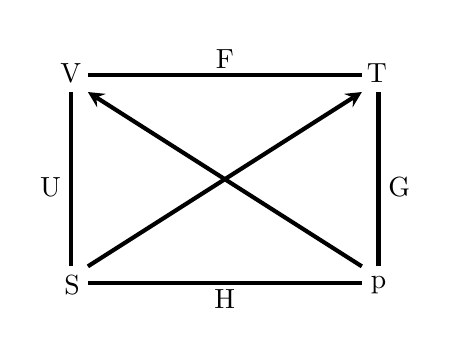
\begin{tikzpicture}
\pgftransformxscale{1.000000}
\pgftransformyscale{-1.000000}
\definecolor{dialinecolor}{rgb}{0.000000, 0.000000, 0.000000}
\pgfsetstrokecolor{dialinecolor}
\definecolor{dialinecolor}{rgb}{1.000000, 1.000000, 1.000000}
\pgfsetfillcolor{dialinecolor}
\definecolor{dialinecolor}{rgb}{1.000000, 1.000000, 1.000000}
\pgfsetfillcolor{dialinecolor}
\fill (29.350000\du,19.800000\du)--(29.350000\du,20.700000\du)--(29.860000\du,20.700000\du)--(29.860000\du,19.800000\du)--cycle;
\pgfsetlinewidth{0.100000\du}
\pgfsetdash{}{0pt}
\pgfsetdash{}{0pt}
\pgfsetmiterjoin
\definecolor{dialinecolor}{rgb}{1.000000, 1.000000, 1.000000}
\pgfsetstrokecolor{dialinecolor}
\draw (29.350000\du,19.800000\du)--(29.350000\du,20.700000\du)--(29.860000\du,20.700000\du)--(29.860000\du,19.800000\du)--cycle;
% setfont left to latex
\definecolor{dialinecolor}{rgb}{0.000000, 0.000000, 0.000000}
\pgfsetstrokecolor{dialinecolor}
\node at (29.605000\du,20.445000\du){p};
\definecolor{dialinecolor}{rgb}{1.000000, 1.000000, 1.000000}
\pgfsetfillcolor{dialinecolor}
\fill (29.600000\du,17.400000\du)--(29.600000\du,18.400000\du)--(30.600000\du,18.400000\du)--(30.600000\du,17.400000\du)--cycle;
\pgfsetlinewidth{0.100000\du}
\pgfsetdash{}{0pt}
\pgfsetdash{}{0pt}
\pgfsetmiterjoin
\definecolor{dialinecolor}{rgb}{1.000000, 1.000000, 1.000000}
\pgfsetstrokecolor{dialinecolor}
\draw (29.600000\du,17.400000\du)--(29.600000\du,18.400000\du)--(30.600000\du,18.400000\du)--(30.600000\du,17.400000\du)--cycle;
% setfont left to latex
\definecolor{dialinecolor}{rgb}{0.000000, 0.000000, 0.000000}
\pgfsetstrokecolor{dialinecolor}
\node at (30.100000\du,18.095000\du){G};
\definecolor{dialinecolor}{rgb}{1.000000, 1.000000, 1.000000}
\pgfsetfillcolor{dialinecolor}
\fill (29.300000\du,14.700000\du)--(29.300000\du,15.600000\du)--(29.827500\du,15.600000\du)--(29.827500\du,14.700000\du)--cycle;
\pgfsetlinewidth{0.100000\du}
\pgfsetdash{}{0pt}
\pgfsetdash{}{0pt}
\pgfsetmiterjoin
\definecolor{dialinecolor}{rgb}{1.000000, 1.000000, 1.000000}
\pgfsetstrokecolor{dialinecolor}
\draw (29.300000\du,14.700000\du)--(29.300000\du,15.600000\du)--(29.827500\du,15.600000\du)--(29.827500\du,14.700000\du)--cycle;
% setfont left to latex
\definecolor{dialinecolor}{rgb}{0.000000, 0.000000, 0.000000}
\pgfsetstrokecolor{dialinecolor}
\node at (29.563750\du,15.345000\du){T};
\definecolor{dialinecolor}{rgb}{1.000000, 1.000000, 1.000000}
\pgfsetfillcolor{dialinecolor}
\fill (21.900000\du,14.700000\du)--(21.900000\du,15.600000\du)--(22.480000\du,15.600000\du)--(22.480000\du,14.700000\du)--cycle;
\pgfsetlinewidth{0.100000\du}
\pgfsetdash{}{0pt}
\pgfsetdash{}{0pt}
\pgfsetmiterjoin
\definecolor{dialinecolor}{rgb}{1.000000, 1.000000, 1.000000}
\pgfsetstrokecolor{dialinecolor}
\draw (21.900000\du,14.700000\du)--(21.900000\du,15.600000\du)--(22.480000\du,15.600000\du)--(22.480000\du,14.700000\du)--cycle;
% setfont left to latex
\definecolor{dialinecolor}{rgb}{0.000000, 0.000000, 0.000000}
\pgfsetstrokecolor{dialinecolor}
\node at (22.190000\du,15.345000\du){V};
\definecolor{dialinecolor}{rgb}{1.000000, 1.000000, 1.000000}
\pgfsetfillcolor{dialinecolor}
\fill (21.950000\du,19.800000\du)--(21.950000\du,20.700000\du)--(22.487500\du,20.700000\du)--(22.487500\du,19.800000\du)--cycle;
\pgfsetlinewidth{0.100000\du}
\pgfsetdash{}{0pt}
\pgfsetdash{}{0pt}
\pgfsetmiterjoin
\definecolor{dialinecolor}{rgb}{1.000000, 1.000000, 1.000000}
\pgfsetstrokecolor{dialinecolor}
\draw (21.950000\du,19.800000\du)--(21.950000\du,20.700000\du)--(22.487500\du,20.700000\du)--(22.487500\du,19.800000\du)--cycle;
% setfont left to latex
\definecolor{dialinecolor}{rgb}{0.000000, 0.000000, 0.000000}
\pgfsetstrokecolor{dialinecolor}
\node at (22.218750\du,20.445000\du){S};
\definecolor{dialinecolor}{rgb}{1.000000, 1.000000, 1.000000}
\pgfsetfillcolor{dialinecolor}
\fill (21.200000\du,17.400000\du)--(21.200000\du,18.400000\du)--(22.200000\du,18.400000\du)--(22.200000\du,17.400000\du)--cycle;
\pgfsetlinewidth{0.100000\du}
\pgfsetdash{}{0pt}
\pgfsetdash{}{0pt}
\pgfsetmiterjoin
\definecolor{dialinecolor}{rgb}{1.000000, 1.000000, 1.000000}
\pgfsetstrokecolor{dialinecolor}
\draw (21.200000\du,17.400000\du)--(21.200000\du,18.400000\du)--(22.200000\du,18.400000\du)--(22.200000\du,17.400000\du)--cycle;
% setfont left to latex
\definecolor{dialinecolor}{rgb}{0.000000, 0.000000, 0.000000}
\pgfsetstrokecolor{dialinecolor}
\node at (21.700000\du,18.095000\du){U};
\definecolor{dialinecolor}{rgb}{1.000000, 1.000000, 1.000000}
\pgfsetfillcolor{dialinecolor}
\fill (25.400000\du,20.100000\du)--(25.400000\du,21.100000\du)--(26.400000\du,21.100000\du)--(26.400000\du,20.100000\du)--cycle;
\pgfsetlinewidth{0.100000\du}
\pgfsetdash{}{0pt}
\pgfsetdash{}{0pt}
\pgfsetmiterjoin
\definecolor{dialinecolor}{rgb}{1.000000, 1.000000, 1.000000}
\pgfsetstrokecolor{dialinecolor}
\draw (25.400000\du,20.100000\du)--(25.400000\du,21.100000\du)--(26.400000\du,21.100000\du)--(26.400000\du,20.100000\du)--cycle;
% setfont left to latex
\definecolor{dialinecolor}{rgb}{0.000000, 0.000000, 0.000000}
\pgfsetstrokecolor{dialinecolor}
\node at (25.900000\du,20.795000\du){H};
\definecolor{dialinecolor}{rgb}{1.000000, 1.000000, 1.000000}
\pgfsetfillcolor{dialinecolor}
\fill (25.400000\du,14.300000\du)--(25.400000\du,15.300000\du)--(26.400000\du,15.300000\du)--(26.400000\du,14.300000\du)--cycle;
\pgfsetlinewidth{0.100000\du}
\pgfsetdash{}{0pt}
\pgfsetdash{}{0pt}
\pgfsetmiterjoin
\definecolor{dialinecolor}{rgb}{1.000000, 1.000000, 1.000000}
\pgfsetstrokecolor{dialinecolor}
\draw (25.400000\du,14.300000\du)--(25.400000\du,15.300000\du)--(26.400000\du,15.300000\du)--(26.400000\du,14.300000\du)--cycle;
% setfont left to latex
\definecolor{dialinecolor}{rgb}{0.000000, 0.000000, 0.000000}
\pgfsetstrokecolor{dialinecolor}
\node at (25.900000\du,14.995000\du){F};
\pgfsetlinewidth{0.100000\du}
\pgfsetdash{}{0pt}
\pgfsetdash{}{0pt}
\pgfsetbuttcap
{
\definecolor{dialinecolor}{rgb}{0.000000, 0.000000, 0.000000}
\pgfsetfillcolor{dialinecolor}
% was here!!!
\definecolor{dialinecolor}{rgb}{0.000000, 0.000000, 0.000000}
\pgfsetstrokecolor{dialinecolor}
\draw (22.600000\du,20.400000\du)--(29.200000\du,20.400000\du);
}
\pgfsetlinewidth{0.100000\du}
\pgfsetdash{}{0pt}
\pgfsetdash{}{0pt}
\pgfsetbuttcap
{
\definecolor{dialinecolor}{rgb}{0.000000, 0.000000, 0.000000}
\pgfsetfillcolor{dialinecolor}
% was here!!!
\definecolor{dialinecolor}{rgb}{0.000000, 0.000000, 0.000000}
\pgfsetstrokecolor{dialinecolor}
\draw (22.200000\du,15.800000\du)--(22.200000\du,20.000000\du);
}
\pgfsetlinewidth{0.100000\du}
\pgfsetdash{}{0pt}
\pgfsetdash{}{0pt}
\pgfsetbuttcap
{
\definecolor{dialinecolor}{rgb}{0.000000, 0.000000, 0.000000}
\pgfsetfillcolor{dialinecolor}
% was here!!!
\definecolor{dialinecolor}{rgb}{0.000000, 0.000000, 0.000000}
\pgfsetstrokecolor{dialinecolor}
\draw (22.600000\du,15.400000\du)--(29.200000\du,15.400000\du);
}
\pgfsetlinewidth{0.100000\du}
\pgfsetdash{}{0pt}
\pgfsetdash{}{0pt}
\pgfsetbuttcap
{
\definecolor{dialinecolor}{rgb}{0.000000, 0.000000, 0.000000}
\pgfsetfillcolor{dialinecolor}
% was here!!!
\definecolor{dialinecolor}{rgb}{0.000000, 0.000000, 0.000000}
\pgfsetstrokecolor{dialinecolor}
\draw (29.600000\du,20.000000\du)--(29.600000\du,15.800000\du);
}
\pgfsetlinewidth{0.100000\du}
\pgfsetdash{}{0pt}
\pgfsetdash{}{0pt}
\pgfsetbuttcap
{
\definecolor{dialinecolor}{rgb}{0.000000, 0.000000, 0.000000}
\pgfsetfillcolor{dialinecolor}
% was here!!!
\pgfsetarrowsend{stealth}
\definecolor{dialinecolor}{rgb}{0.000000, 0.000000, 0.000000}
\pgfsetstrokecolor{dialinecolor}
\draw (22.600000\du,20.000000\du)--(29.200000\du,15.800000\du);
}
\pgfsetlinewidth{0.100000\du}
\pgfsetdash{}{0pt}
\pgfsetdash{}{0pt}
\pgfsetbuttcap
{
\definecolor{dialinecolor}{rgb}{0.000000, 0.000000, 0.000000}
\pgfsetfillcolor{dialinecolor}
% was here!!!
\pgfsetarrowsend{stealth}
\definecolor{dialinecolor}{rgb}{0.000000, 0.000000, 0.000000}
\pgfsetstrokecolor{dialinecolor}
\draw (29.200000\du,20.000000\du)--(22.600000\du,15.800000\du);
}
\end{tikzpicture}

	\end{minipage}
	\begin{minipage}{0.65 \columnwidth}
		\begin{itemize}
			\item The derivative of a potential (edge) with respect to a variable (corner) is given by the variable at the diagonally opposite corner. The arrows in the diagonals determine the sign. \\
			\item For the Maxwell relations, derivatives of variables along an edge of the quadrangle, at constant variable in the diagonally opposite corner, are just equal to the corresponding derivative on the other side.
		\end{itemize}
	\end{minipage}
	
	\setlength{\abovedisplayskip}{0pt}
	\setlength{\belowdisplayskip}{0pt}
	\setlength{\abovedisplayshortskip}{0pt}
	\setlength{\belowdisplayshortskip}{0pt}
	\begin{align*}
		& \evalb{\pder{V}{T}}_p = \alpha V	\tag*{Definition of the isobaric expansion ceofficient $\alpha$ (GNS 4.141)} \\
		& \evalb{\pder{V}{p}}_T = -V \kappa \tag*{Defintion of the isothermal compressibility $\kappa$ (GNS 4.143)} \\		
		& C_p = C_V +TV\frac{\alpha^2}{\kappa}	\tag*{Relationship between $C_p$ and $C_V$ (GNS Ex. 4.12)} \\
	& \small \hspace{-10pt} \textbf{Number of Microstates $\Omega$ and Entropy $S$} \small \\	
		& \sigma(E) = \int_{E=H(q,p)} d\sigma	\tag*{Surface area of energy hypersurface (GNS 5.7)} \\
		& \omega(E,V,N) = \int_{H(q_\nu, p_\nu) \leq E} d^{3N}q \; d^{3N} p	\tag*{Total phase-space volume (GNS 5.9)} \\
		& \Omega(E,V,N) = \frac{\sigma(E,V,N)}{\sigma_0} = \frac{1}{\sigma_0} \pder{\omega}{E}	\tag*{Microstates of distiguishable particles (GNS 5.13)} \\
		& S = k \ln \Omega(E,V,N)	\tag*{Statistical defintion of entropy (GNS 5.23)} \\
		& \Omega(E,V,N) = \frac{1}{N!} \frac{\sigma(E,V,N)}{\sigma_0}	\tag*{Microstates of indistiguishable particles (GNS 5.43)} \\
		& S(E,V,N) = Nk \lrc{\frac{5}{2} + \ln \lrb{\frac{V}{N h^3} \lrp{\frac{4 \pi m E}{3N}}^{3/2}}}	\tag*{Sackur-Tetrode Equation (GNS 5.63)} \\
		& \Omega(E,V,N) = g(E,V,N) E	\tag*{Number of microstates from density of states (GNS 5.65)} \\
		& g(E) = \pder{\Sigma(E)}{E}	\tag*{Definition of the density of states (GNS 5.65)} \\
		& \Sigma(E) = \frac{1}{N! h^{3N}} \int_{H(q_\nu,p_\nu) \leq E} d^{3N}p \; d^{3N}q	\tag*{Number of microstates in energy sphere (GNS 5.65)} \\
		& \lambda = \lrp{\frac{h^2}{2 \pi mkT}}^{1/2}	\tag*{Thermal wavelength (GNS pg. 140)} \\
	& \small \hspace{-10pt} \textbf{Ensemble Theory and Microcanonical Ensembles} \small \\
		& \expval{f} =  \frac{1}{h^{3N}}\int d^{3N} q \; d^{3N} p \; f(q_\nu,p_\nu) \rho (q_\nu, p_{\nu})	\tag*{Definition of the ensemble average (GNS 6.8)} \\
		& \rho_{\text{mc}} = \begin{cases}
			\frac{1}{\Omega} & E \leq H(q_v,p_v) \leq E + \Delta E \\
			0	& \text{otherwise} \\
		\end{cases}	\tag*{Phase-space density of microcanonical ensemble (GNS 6.9)} \\
		& \tder{\rho}{t} = \pder{\rho}{t} + \{ p,H \} = 0	\tag*{Liouville's theorem (6.18)} \\
		& S = \expval{-k \ln \rho}	\tag*{Entropy as an ensemble average (GNS 6.37)} \\
	\end{align*} \newpage
	\setlength{\abovedisplayskip}{-25pt}
	\setlength{\belowdisplayskip}{-10pt}
	\setlength{\abovedisplayshortskip}{0pt}
	\setlength{\belowdisplayshortskip}{0pt}
	\begin{align*} 
	& \small \hspace{-10pt} \textbf{The Canonical Ensemble} \small \\
		& \rho_c(q_\nu,p_\nu) = \frac{\exp\{ - \beta H(q_\nu,p_\nu ) \}}{h^{-3N} \int d^{3N}q \; d^{3N}p \; \exp \{ -\beta H(q_\nu, p_\nu) \}}	\tag*{Canonical phase-space density (GNS 7.9)} \\
		& Z = \sum_i \exp \{ - \beta E_i \}	\tag*{Canonical partition function (GNS 7.22)} \\
		& Z = \frac{1}{h^{3N}} \int d^{3N}q \; d^{3N}p \; \exp{-\beta H(q_\nu,p_\nu)}	\tag*{Continuous partition funciton (GNS 7.24)} \\
		& F(T,V,N) = -kT \ln Z(T,V,N)	\tag*{Free energy from the partition function (GNS 7.35)} \\
		& Z(\beta) = \int_0^\infty dE \; g(E) e^{-\beta E}	\tag*{Canonical partition function from microcanonical density of states (GNS 7.103)} \\
		& g(E) = \frac{1}{2 \pi i} \int_{\beta'-i \infty}^{\beta'+i \infty} d \beta \; e^{\beta E} Z(\beta)	\tag*{Microcanonical density of states from partition function (GNS 7.107)} \\
		& \expval{T} = - \frac{1}{2} \expval{\sum_{i=1}^N \ve{r}_i \cdot \ve{F}_i} = \frac{3}{2} NkT	\tag*{The virial theorem (GNS 7.149)} \\
		& \expval{H} = \frac{1}{2} kT	\tag*{Equipartition theorem (GNS 7.156)} \\
	& \small \hspace{-10pt} \textbf{Applications of Boltzmann Statistics} \small \\
		& \chi =N \frac{g^2 \mu_B^2 j(j+1)}{3kT} = \frac{C}{T}	\tag*{Magnetic susceptibility from the Curie law (GNS 8.52)} \\
		& C = Nk \lrp{\frac{2 \mu_B H}{kT}}^2 \exp \lrc{\frac{2 \mu_B H}{kT}} \lrp{1 + \exp\lrc{\frac{2 \mu_B H}{kT}}}^{-2}		\tag*{Schottky heat cap. (GNS 8.60)} \\
	& \small \hspace{-10pt} \textbf{The Macrocanonical Ensemble} \small \\
		& \rho_{gc}(N, q_\nu, p_\nu) = \frac{\exp \{ -\beta(H(q_\nu, p_\nu) -\mu N) \}}{\sum_{N=0}^{\infty} h^{-3N} \int d^{3N} q \int d^{3N}p \; \exp \{ -\beta(H(q_\nu, p_\nu) -\mu N) \}} \tag*{Grand canonical phase-space density (GNS 9.11)} \\
		& \mathcal{Z} = \sum_{N=0}^{\infty} \frac{1}{h^{3N}} \int d^{3N}q  \int d^{3N}p \; \exp \{ -\beta(H(q_\nu, p_\nu) -\mu N) \}	\tag*{Grand canonical partition function (GNS 9.27)} \\
		& \phi(T,V,\mu) = -kT \ln \mathcal{Z}(T,V,\mu)	\tag*{Macrocanonical potential (GNS 9.38)} \\
		& \mathcal{Z}(T,V,\mu) = \sum_{N=0}^{\infty} \lrp{\exp\lrc{\frac{\mu}{kT}}}^N Z(T,V,N)	\tag*{Relation between canonical and grand canonical partition functions (GNS 9.40)} \\
	\end{align*}
	
\end{multicols}
% --------------------------------------------------------------
%     You don't have to mess with anything below this line.
% --------------------------------------------------------------
 
\end{document}
